\section{eo\-External\-EO$<$ Fit, External $>$ Class Template Reference}
\label{classeo_external_e_o}\index{eoExternalEO@{eoExternalEO}}
Definition of an object that allows an external struct to be inserted in {\bf EO}{\rm (p.\,\pageref{class_e_o})}.  


{\tt \#include $<$eo\-External\-EO.h$>$}

Inheritance diagram for eo\-External\-EO$<$ Fit, External $>$::\begin{figure}[H]
\begin{center}
\leavevmode
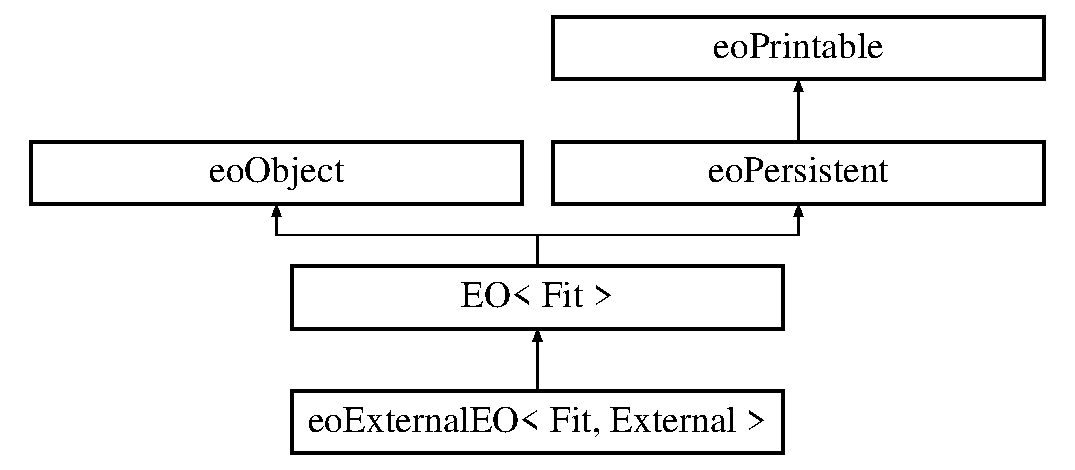
\includegraphics[height=4cm]{classeo_external_e_o}
\end{center}
\end{figure}
\subsection*{Public Member Functions}
\begin{CompactItemize}
\item 
{\bf eo\-External\-EO} (const External \&ext)\label{classeo_external_e_o_a1}

\begin{CompactList}\small\item\em Init external\-Eo with the struct itself and set fitness to zero. \item\end{CompactList}\item 
{\bf eo\-External\-EO} (std::istream \&is, const External \&ext)\label{classeo_external_e_o_a2}

\item 
virtual void {\bf read\-From} (std::istream \&\_\-is)\label{classeo_external_e_o_a3}

\begin{CompactList}\small\item\em Read object, the external struct needs to have an operator$>$$>$ defined. \item\end{CompactList}\item 
virtual void {\bf print\-On} (std::ostream \&\_\-os) const 
\begin{CompactList}\small\item\em Write object. \item\end{CompactList}\end{CompactItemize}


\subsection{Detailed Description}
\subsubsection*{template$<$class Fit, class External$>$ class eo\-External\-EO$<$ Fit, External $>$}

Definition of an object that allows an external struct to be inserted in {\bf EO}{\rm (p.\,\pageref{class_e_o})}. 

This struct or class can be of any form, the only thing this class does is attach a fitness value to it and makes it the appropriate type (derives it from {\bf EO}{\rm (p.\,\pageref{class_e_o})}). 



Definition at line 39 of file eo\-External\-EO.h.

\subsection{Member Function Documentation}
\index{eoExternalEO@{eo\-External\-EO}!printOn@{printOn}}
\index{printOn@{printOn}!eoExternalEO@{eo\-External\-EO}}
\subsubsection{\setlength{\rightskip}{0pt plus 5cm}template$<$class Fit, class External$>$ virtual void {\bf eo\-External\-EO}$<$ Fit, External $>$::print\-On (std::ostream \& {\em \_\-os}) const\hspace{0.3cm}{\tt  [inline, virtual]}}\label{classeo_external_e_o_a4}


Write object. 

Called print\-On since it prints the object \_\-on\_\- a stream. \begin{Desc}
\item[Parameters:]
\begin{description}
\item[{\em \_\-os}]A std::ostream. \end{description}
\end{Desc}


Reimplemented from {\bf EO$<$ Fit $>$} {\rm (p.\,\pageref{class_e_o_z10_2})}.

Definition at line 69 of file eo\-External\-EO.h.

References EO$<$ F $>$::print\-On().

The documentation for this class was generated from the following file:\begin{CompactItemize}
\item 
eo\-External\-EO.h\end{CompactItemize}
